% -*- TeX-engine: luatex -*-
% The research talk will be for 40 minutes and should be at a level
% suitable to a general audience with expertise in Applied &
% Computational Mathematics and include some aspects of your research.
% I would suggest that you aim to spend 10-15 minutes on the
% background and general context of the research, leading up to an
% account of your own contribution to the field and an indication of
% its significance. During your visit to our School you will of course
% have the opportunity to discuss your work in greater depth with some
% of our faculty.

%
% Background: finite element methods, automation (assembly)
% Preconditioning: optimal algorithms, composable implementation
% Significance: first general implementation of many state-of-the-art
% multigrid smoothers

\documentclass[presentation,aspectratio=43, 10pt]{beamer}
\usepackage{pifont}
\newcommand{\cmark}{\ding{51}}
\newcommand{\xmark}{\ding{55}}

\usepackage{booktabs}
% \titlegraphic{\hfill
\includegraphics[height=1.25cm]{durham-logo}}
\usepackage{appendixnumberbeamer}
\def\xunderbrace#1_#2{{\underbrace{#1}_{\mathclap{#2}}}}
\def\xoverbrace#1^#2{{\overbrace{#1}^{\mathclap{#2}}}}
\def\xunderarrow#1_#2{{\underset{\overset{\uparrow}{\mathclap{#2}}}{#1}}}
\def\xoverarrow#1^#2{{\overset{\underset{\downarrow}{\mathclap{#2}}}{#1}}}
\usepackage{amsmath}
\usepackage{amssymb}
\usepackage{mathtools}
\usepackage{hyperref}
\usepackage{xspace}
\newcommand{\arxivlink}[2]{{\texttt{arXiv:\,\href{https://arxiv.org/abs/#1}{#1\,[#2]}}}}

\newcommand{\honev}{\ensuremath{{H}^1(\Omega; \mathbb{R}^d)}\xspace}
\newcommand{\ltwov}{\ensuremath{{L}^2(\Omega; \mathbb{R}^d)}\xspace}
\newcommand{\ltwo}{\ensuremath{{L}^2(\Omega)}\xspace}
\newcommand{\inner}[1]{\left\langle #1 \right \rangle}
\newcommand{\advect}[2]{\ensuremath{(#2 \cdot \nabla) #1}}
\newcommand{\kerdiv}{\ker\div}
\newcommand{\eps}[1]{\ensuremath{\varepsilon{(#1)}}}
\newcommand{\kercurl}{\ker\curl}
\newcommand{\dx}{\ \text{d}x}
\newcommand{\ds}{\ \text{d}s}
\newcommand{\Pq}{\ensuremath{\mathrm{P}_{Q_h}}}
\newcommand{\PqK}{\ensuremath{\mathrm{P}_{Q_h(K)}}}
\newcommand{\Ptwo}{\ensuremath{\mathbb{P}_2}\xspace}
\newcommand{\Pthree}{\ensuremath{\mathbb{P}_3}\xspace}
\newcommand{\PtwoPzero}{\ensuremath{[\mathbb{P}_2]^2\mathrm{-}\mathbb{P}_0}\xspace}
\newcommand{\PtwothreePzero}{\ensuremath{[\mathbb{P}_2]^3\mathrm{-}\mathbb{P}_0}\xspace}
\newcommand{\PthreePzero}{\ensuremath{[\mathbb{P}_3]^3\mathrm{-}\mathbb{P}_0}\xspace}
\newcommand{\Pzero}{\ensuremath{\mathbb{P}_0}\xspace}
\newcommand{\Pv}{\ensuremath{\mathbb{P}_v}\xspace}
\newcommand{\BR}{\ensuremath{\left[\mathbb{P}_1 \oplus B^F_3\right]}\xspace}
\newcommand{\PoneFB}{\ensuremath{\mathbb{P}_1 \oplus B^F_3}\xspace}
\newcommand{\PtwoFB}{\ensuremath{\mathbb{P}_2 \oplus B^F_3}\xspace}
\newcommand{\BRzero}{\ensuremath{\BR^3\mathrm{-}\mathbb{P}_0}\xspace}
\newcommand{\fmw}{\ensuremath{\left(\mathbb{P}_2 \oplus B^F_3\right)}\xspace}
\newcommand{\fmwzero}{\ensuremath{\fmw^3\mathrm{-}\mathbb{P}_0}\xspace}
\setbeamersize{text margin left=0.5cm, text margin right=0.5cm}
\let\Re\relax
\DeclareMathOperator{\Re}{Re}


\usepackage{minted}
\usepackage[url=false,
doi=true,
isbn=false,
style=authoryear,
maxnames=5,
giveninits=true,
uniquename=init,
backend=biber]{biblatex}
\renewcommand{\bibfont}{\fontsize{7}{7}\selectfont}
\addbibresource{../literature.bib}
\setbeamertemplate{bibliography item}[triangle]
\defbibenvironment{bibliography}
  {\list{}
     {\settowidth{\labelwidth}{\usebeamertemplate{bibliography item}}%
      \setlength{\leftmargin}{\labelwidth}%
      \setlength{\rightmargin}{\labelwidth}%
      \setlength{\labelsep}{\biblabelsep}%
      \addtolength{\leftmargin}{\labelsep}%
      \setlength{\itemsep}{\bibitemsep}%
      \setlength{\parsep}{\bibparsep}}}
  {\endlist}
  {\item}
\setlength{\bibitemsep}{1ex}
\setlength{\fboxsep}{1pt}

\renewbibmacro{in:}{}
\DeclareFieldFormat[article]{volume}{\textbf{#1}}
\DeclareFieldFormat{doi}{%
  doi\addcolon%
  {\scriptsize\ifhyperref{\href{http://dx.doi.org/#1}{\nolinkurl{#1}}}
    {\nolinkurl{#1}}}}
\AtEveryBibitem{%
\clearfield{pages}%
\clearfield{issue}%
\clearfield{number}%
}

\DeclareMathOperator{\grad}{grad}
\let\div\relax
\DeclareMathOperator{\div}{div}
\DeclareMathOperator{\curl}{curl}
\DeclareMathOperator{\range}{range}
\DeclareMathOperator{\sym}{sym}
\usetheme{metropolis}
\setbeamertemplate{title graphic}{
  \vbox to 0pt {
    \vspace*{1em}
    \inserttitlegraphic%
  }%
  \nointerlineskip%
}
\metroset{background=light,progressbar=frametitle,numbering=counter,block=fill}

% https://www.dur.ac.uk/marketingandcommunications/marketing/branding/colourpalette/
% Most of these are indistinguishable to those suffering colour blindness
\definecolor{purple}{HTML}{68246D}
\definecolor{blue}{HTML}{002A41}
\definecolor{red}{HTML}{BE1E2D}
\definecolor{cyan}{HTML}{00AEEF}
\definecolor{yellow}{HTML}{00AA1A}

\newenvironment{variableblock}[3]
{\setbeamercolor{block body}{#2}
\setbeamercolor{block title}{#3}
\begin{block}{#1}}%
{\end{block}}
  
\newenvironment{challenge}[1]%
{\begin{variableblock}{#1}{bg=red!20,fg=black}{bg=red,fg=white}}%
{\end{variableblock}}

\newenvironment{answer}[1]%
{\begin{variableblock}{#1}{bg=cyan!20,fg=black}{bg=cyan,fg=white}}%
{\end{variableblock}}

\renewenvironment{exampleblock}[1]%
{\begin{variableblock}{#1}{bg=yellow!20,fg=black}{bg=yellow,fg=white}}%
{\end{variableblock}}

\setbeamercolor{normal text}{
  fg=black,
  bg=white
}
\setbeamercolor{alerted text}{
  fg=red
}
\setbeamercolor{example text}{
  fg=blue
}

\setbeamercolor{palette primary}{%
  use=normal text,
  fg=normal text.bg,
  bg=purple,
}

\usetheme{metropolis}

\author{Lawrence Mitchell\inst{1,*}
  \\ {\scriptsize C.J.~Cotter, P.E.~Farrell, T.H.~Gibson, D.A.~Ham,
    P.H.J.~Kelly, R.C.~Kirby, M.G.~Knepley, E.H.~M\"uller,
    F.~Wechsung,  \dots}}
\institute{
  \inst{1}Department of Computer Science, Durham University\\
  \inst{*}\texttt{lawrence.mitchell@durham.ac.uk}}

\date{6th January 2020}
\title{From symbolic mathematics to fast solvers for finite element problems}

\usepackage{tikz}
\usetikzlibrary{trees,calc,positioning}
\usetikzlibrary{shapes, shapes.geometric}
\usetikzlibrary{arrows,chains,positioning,fit,backgrounds,calc,shapes,
  shadows,scopes,decorations.markings,plotmarks}

\usepackage{pgf}
\usepackage{pgfplots}
\usepackage{pgfplotstable}

\newcommand*{\tettextsize}{\footnotesize}
\tikzstyle{line} = [draw, -, thick]
\tikzstyle{nodraw} = [draw, fill, circle, minimum width=0pt, inner sep=0pt]
\tikzstyle{sieve} = [line, circle, font=\tettextsize, inner sep=0pt,
  minimum size=12pt]

\tikzstyle{cell} = [sieve, fill=blue!60]
\tikzstyle{facet} = [sieve, fill=green!35]
\tikzstyle{edge} = [sieve, fill=red!35]
\tikzstyle{vertex} = [sieve, fill=blue!35]

% https://tex.stackexchange.com/questions/27171/padded-boundary-of-convex-hull
\newcommand{\convexpath}[2]{
  [
  create hullcoords/.code={
    \global\edef\namelist{#1}
    \foreach [count=\counter] \nodename in \namelist {
      \global\edef\numberofnodes{\counter}
      \coordinate (hullcoord\counter) at (\nodename);
    }
    \coordinate (hullcoord0) at (hullcoord\numberofnodes);
    \pgfmathtruncatemacro\lastnumber{\numberofnodes+1}
    \coordinate (hullcoord\lastnumber) at (hullcoord1);
  },
  create hullcoords
  ]
  ($(hullcoord1)!#2!-90:(hullcoord0)$)
  \foreach [
  evaluate=\currentnode as \previousnode using \currentnode-1,
  evaluate=\currentnode as \nextnode using \currentnode+1
  ] \currentnode in {1,...,\numberofnodes} {
    let \p1 = ($(hullcoord\currentnode) - (hullcoord\previousnode)$),
    \n1 = {atan2(\y1,\x1) + 90},
    \p2 = ($(hullcoord\nextnode) - (hullcoord\currentnode)$),
    \n2 = {atan2(\y2,\x2) + 90},
    \n{delta} = {Mod(\n2-\n1,360) - 360}
    in
    {arc [start angle=\n1, delta angle=\n{delta}, radius=#2]}
    -- ($(hullcoord\nextnode)!#2!-90:(hullcoord\currentnode)$)
  }
}

\graphicspath{{./\jobname.figures/}{../pictures/}}

\begin{document}

\maketitle

\begin{frame}
  \frametitle{Outline}

  \begin{itemize}
  \item Overview
    \begin{itemize}
    \item Automated finite elements
    \item Multigrid preconditioning for numerical weather prediction
    \end{itemize}
  \item In depth
    \begin{itemize}
    \item Parameter-robust preconditioning for the Navier--Stokes equations
    \end{itemize}
  \item Future directions
  \end{itemize}
\end{frame}

\section{Automated finite elements}

\begin{frame}[fragile]
  \frametitle{Code that captures mathematical structure}
  \begin{columns}
    \begin{column}{0.5\framewidth}
      {\footnotesize
        Find $(u, p, T) \in V\times W\times Q$ s.t.
        \begin{align*}
          \int\!\nabla u \cdot \nabla v + (u \cdot \nabla u) \cdot v \\
          - p\nabla\cdot v + \frac{\text{Ra}}{\text{Pr}} Tg \hat{z} \cdot v\,\text{d}x &= 0 \\
          \int\!\nabla\cdot u q\,\text{d}x&= 0\\
          \int\! (u\cdot \nabla T) S + \text{Pr}^{-1} \nabla T \cdot \nabla
          S\,\text{d}x &= 0\\
          \quad \forall\, (v,q,T) \in V\times W \times Q
        \end{align*}
        }
    \end{column}
      \begin{column}{0.5\framewidth}
\begin{minted}[fontsize=\scriptsize]{python}
from firedrake import *
mesh = Mesh(...)
V = VectorFunctionSpace(mesh, "CG", 2)
W = FunctionSpace(mesh, "CG", 1)
Q = FunctionSpace(mesh, "CG", 1)
Z = V * W * Q
Ra = Constant(...)
Pr = Constant(...)
upT = Function(Z)
u, p, T = split(upT)
v, q, S = TestFunctions(Z)
bcs = [...]

F = (inner(grad(u), grad(v))
     + inner(dot(grad(u), u), v)
     - inner(p, div(v))
     + (Ra/Pr)*inner(T*g, v)
     + inner(div(u), q)
     + inner(dot(grad(T), u), S)
     + (1/Pr)*inner(grad(T), grad(S)))*dx

solve(F == 0, upT, bcs=bcs)
\end{minted}
      \end{column}
  \end{columns}
\end{frame}

\begin{frame}
  \frametitle{The computer should work for \emph{you}}
  \begin{itemize}
  \item Mathematics just says ``here is the integral to compute on each
    element, do that everywhere''
  \item Code specifies an \emph{implementation}
  \end{itemize}
  \begin{block}{Assertion(s)}
    Having chosen a discretisation, writing the element integral is ``mechanical''.

    With an element integral in hand, integrating over a mesh is
    ``mechanical''.
  \end{block}

  \begin{corollary}
    Computers are good at mechanical things, why don't we get the
    computer to write them for us?
  \end{corollary}
\end{frame}

\begin{frame}
  \frametitle{Firedrake \url{www.firedrakeproject.org}}
  \begin{columns}
    \begin{column}{0.8\textwidth}
      \begin{quote}
        {\normalfont [\ldots]} an automated system for the solution of
        partial differential equations using the finite element
        method.
      \end{quote}
    \end{column}
    \begin{column}{0.2\textwidth}
      
\includegraphics[width=0.8\textwidth]{firedrake}
    \end{column}
  \end{columns}
  \begin{overlayarea}{\textwidth}{0.6\textheight}
    \begin{onlyenv}<1>
      \begin{itemize}
      \item Written in Python.
      \item Finite element problems specified with \emph{embedded}
        domain specific language, UFL \parencite{Alnaes:2014} from the
        FEniCS project.
      \item Domain-specifc optimising compiler.
      \item \emph{Runtime} compilation to optimised, low-level (C)
        code.
      \end{itemize}
      \begin{flushright}
        {\scriptsize F.~Rathgeber, D.A.~Ham, \textbf{L.~Mitchell}, M.~Lange,
        F.~Luporini, A.T.T.~McRae, G.-T.~Bercea, G.R.~Markall,
        P.H.J.~Kelly. ACM Transactions on Mathematical Software
        (2016). \arxivlink{1501.01809}{cs.MS}\nocite{Rathgeber:2016}}
      \end{flushright}
  \end{onlyenv}
  \begin{onlyenv}<2>
    \begin{block}{User groups at}
      Imperial, Oxford, Bath, Leeds, Durham, Kiel, Rice, Houston,
      Exeter, Buffalo, Waterloo, Washington, Baylor, Edinburgh, \dots

      Fourth annual (and first USA) user meeting this February (Seattle).
    \end{block}
  \end{onlyenv}
\end{overlayarea}
\end{frame}

\begin{frame}
  \frametitle{Application: coastal ocean modelling}
  \begin{columns}
    \begin{column}{0.55\textwidth}
      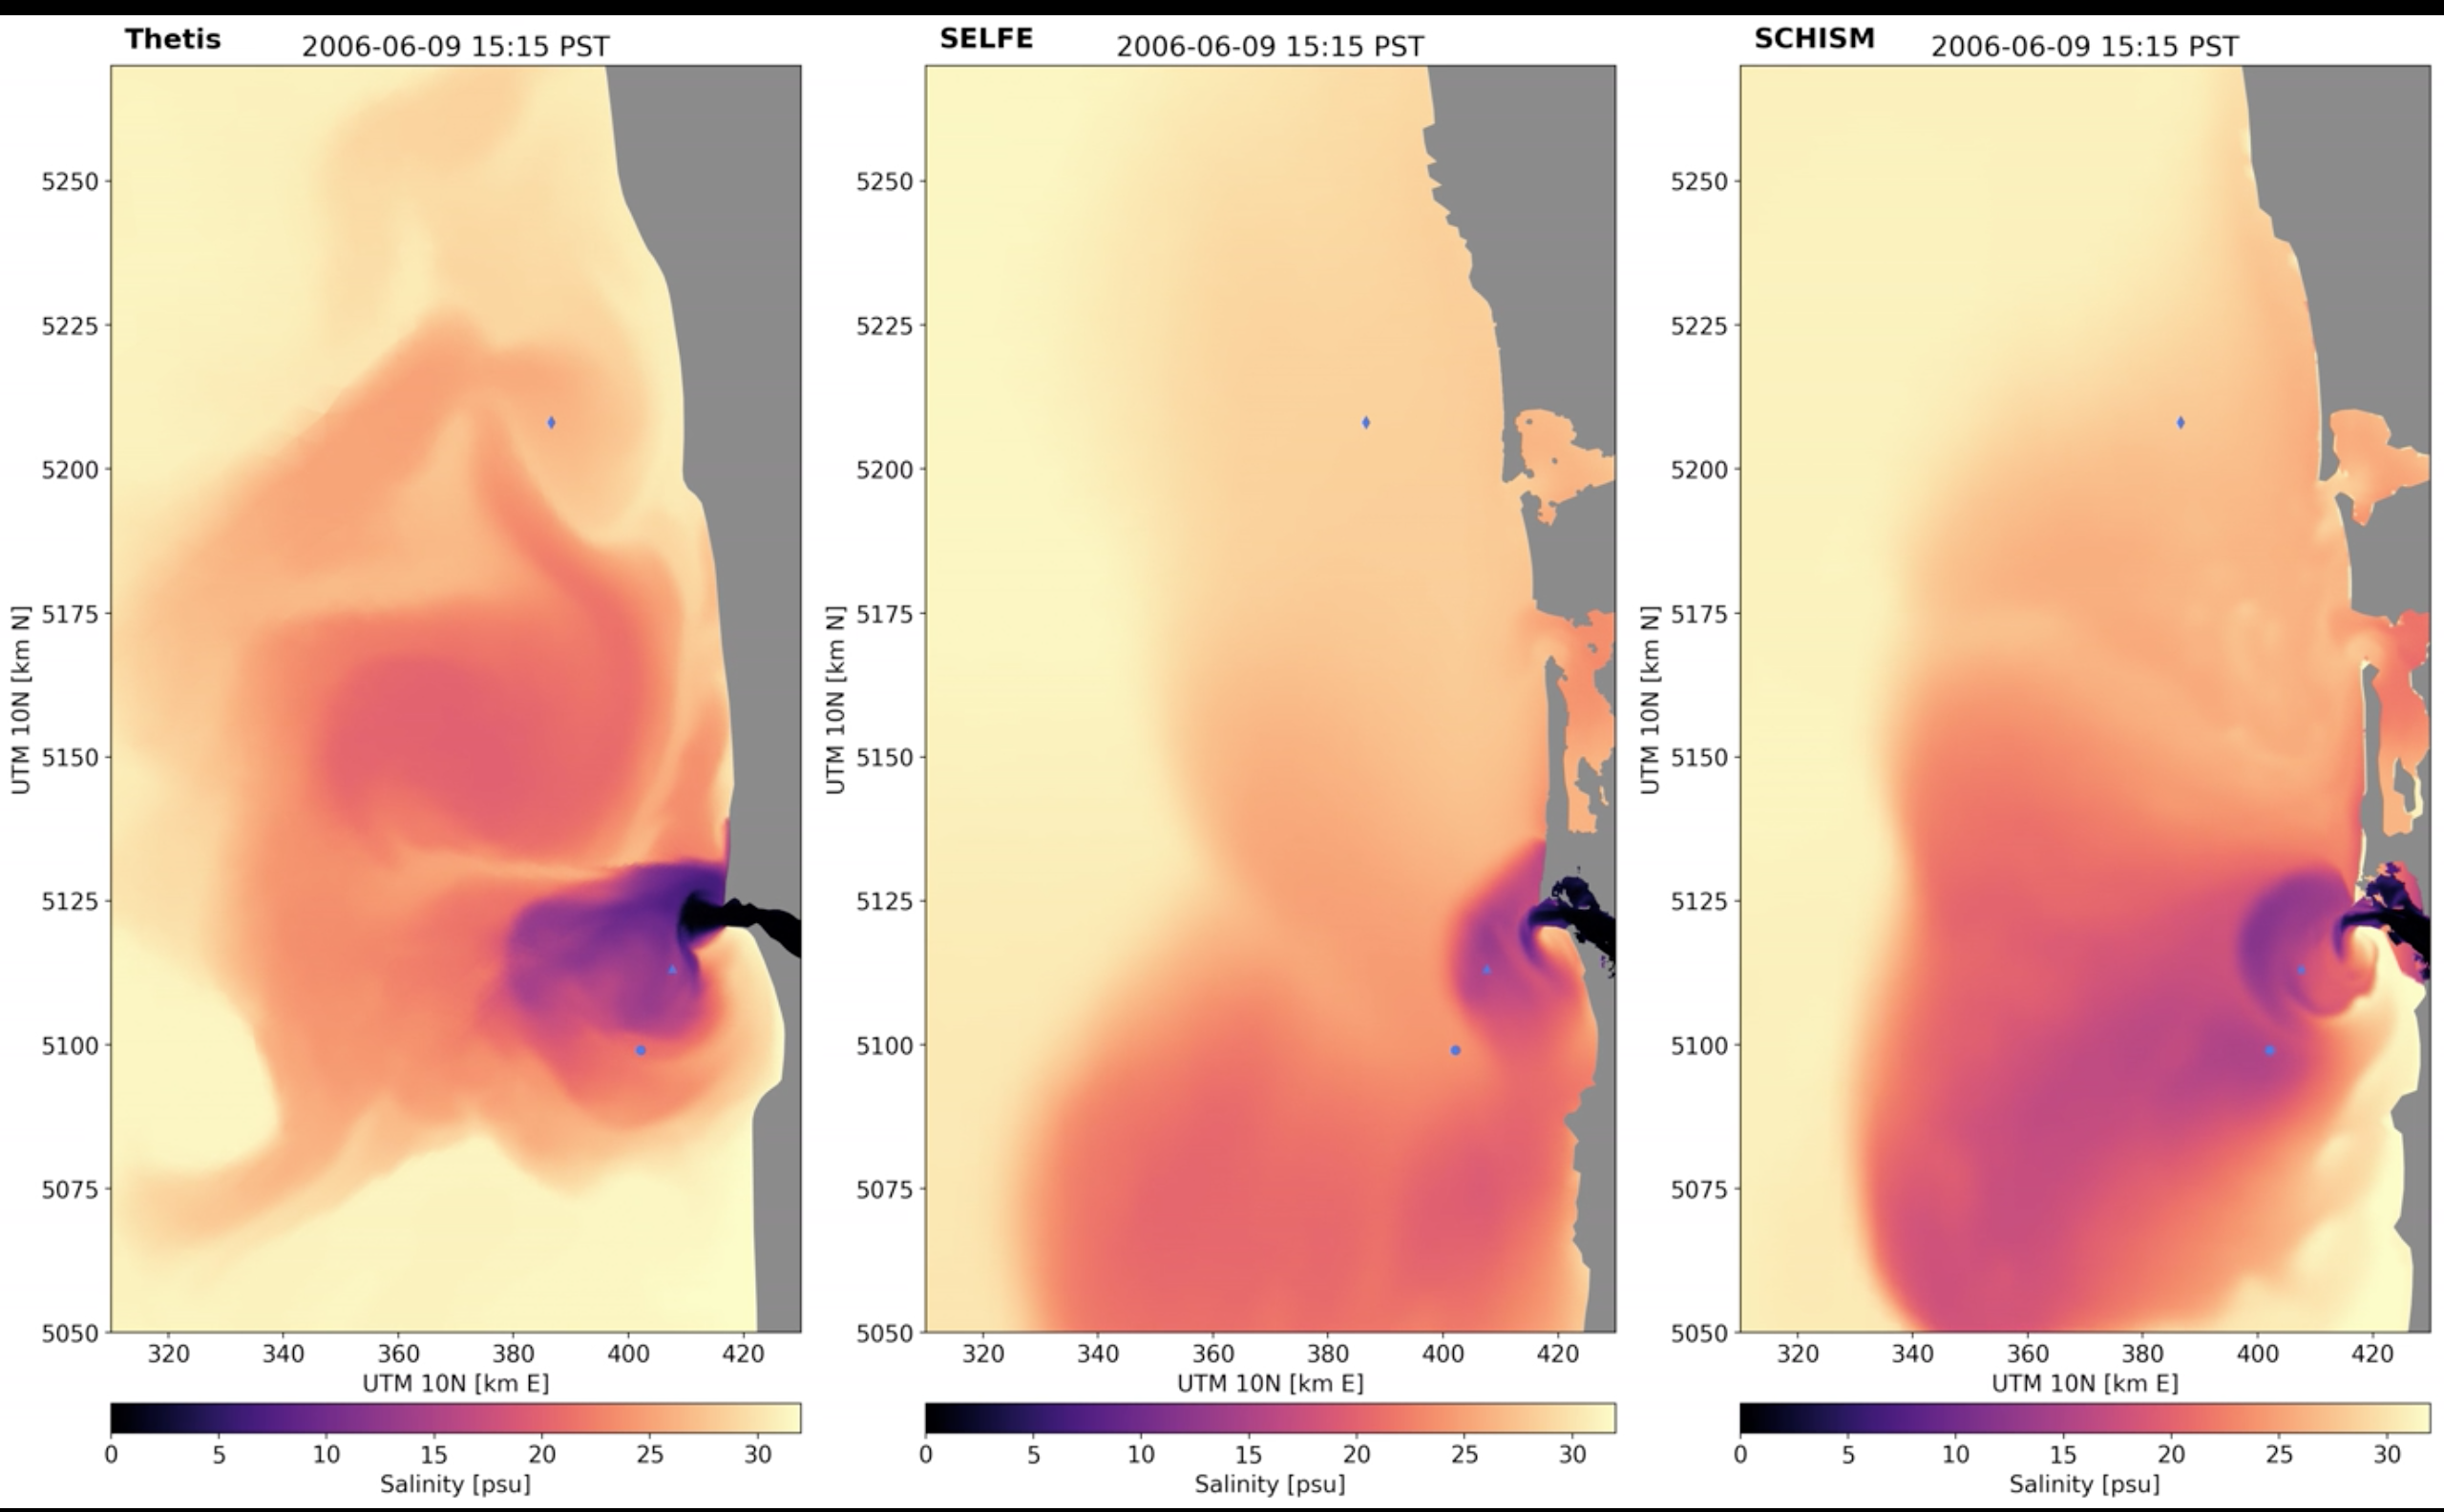
\includegraphics[height=0.45\textheight]{thetis-snapshot}

      {\tiny Surface salinity of the Columbia river plume. Credit
        T.~K\"arn\"a, Finnish Meteorological Institute}
    \end{column}
    \hspace{-0.04\textwidth}
    \begin{column}{0.48\textwidth}
      \begin{itemize}
      \item Lower numerical mixing, improved results.
      \item 3-8x faster than models with similar quality of results.
      \item Differentiable: efficient adjoint.
      \item Used at Finnish Met Institute; Earth Sciences at
        Imperial; Institute for Infrastructure and Environment (here).
      \item \url{thetisproject.org}
       \end{itemize}
    \end{column}
  \end{columns}
  \begin{flushright}
    {\scriptsize T.~K\"arn\"a, S.C.~Kramer, \textbf{L.~Mitchell}, D.A.~Ham,
      M.D.~Piggott, A.M.~Baptista. Geoscientific Model Development
      (2018).
      \arxivlink{1711.08552}{physics.ao-ph}\nocite{Karna:2018}}
  \end{flushright}
\end{frame}

\begin{frame}
  \frametitle{Application: numerical weather prediction}
  \begin{columns}
    \begin{column}{3cm}
      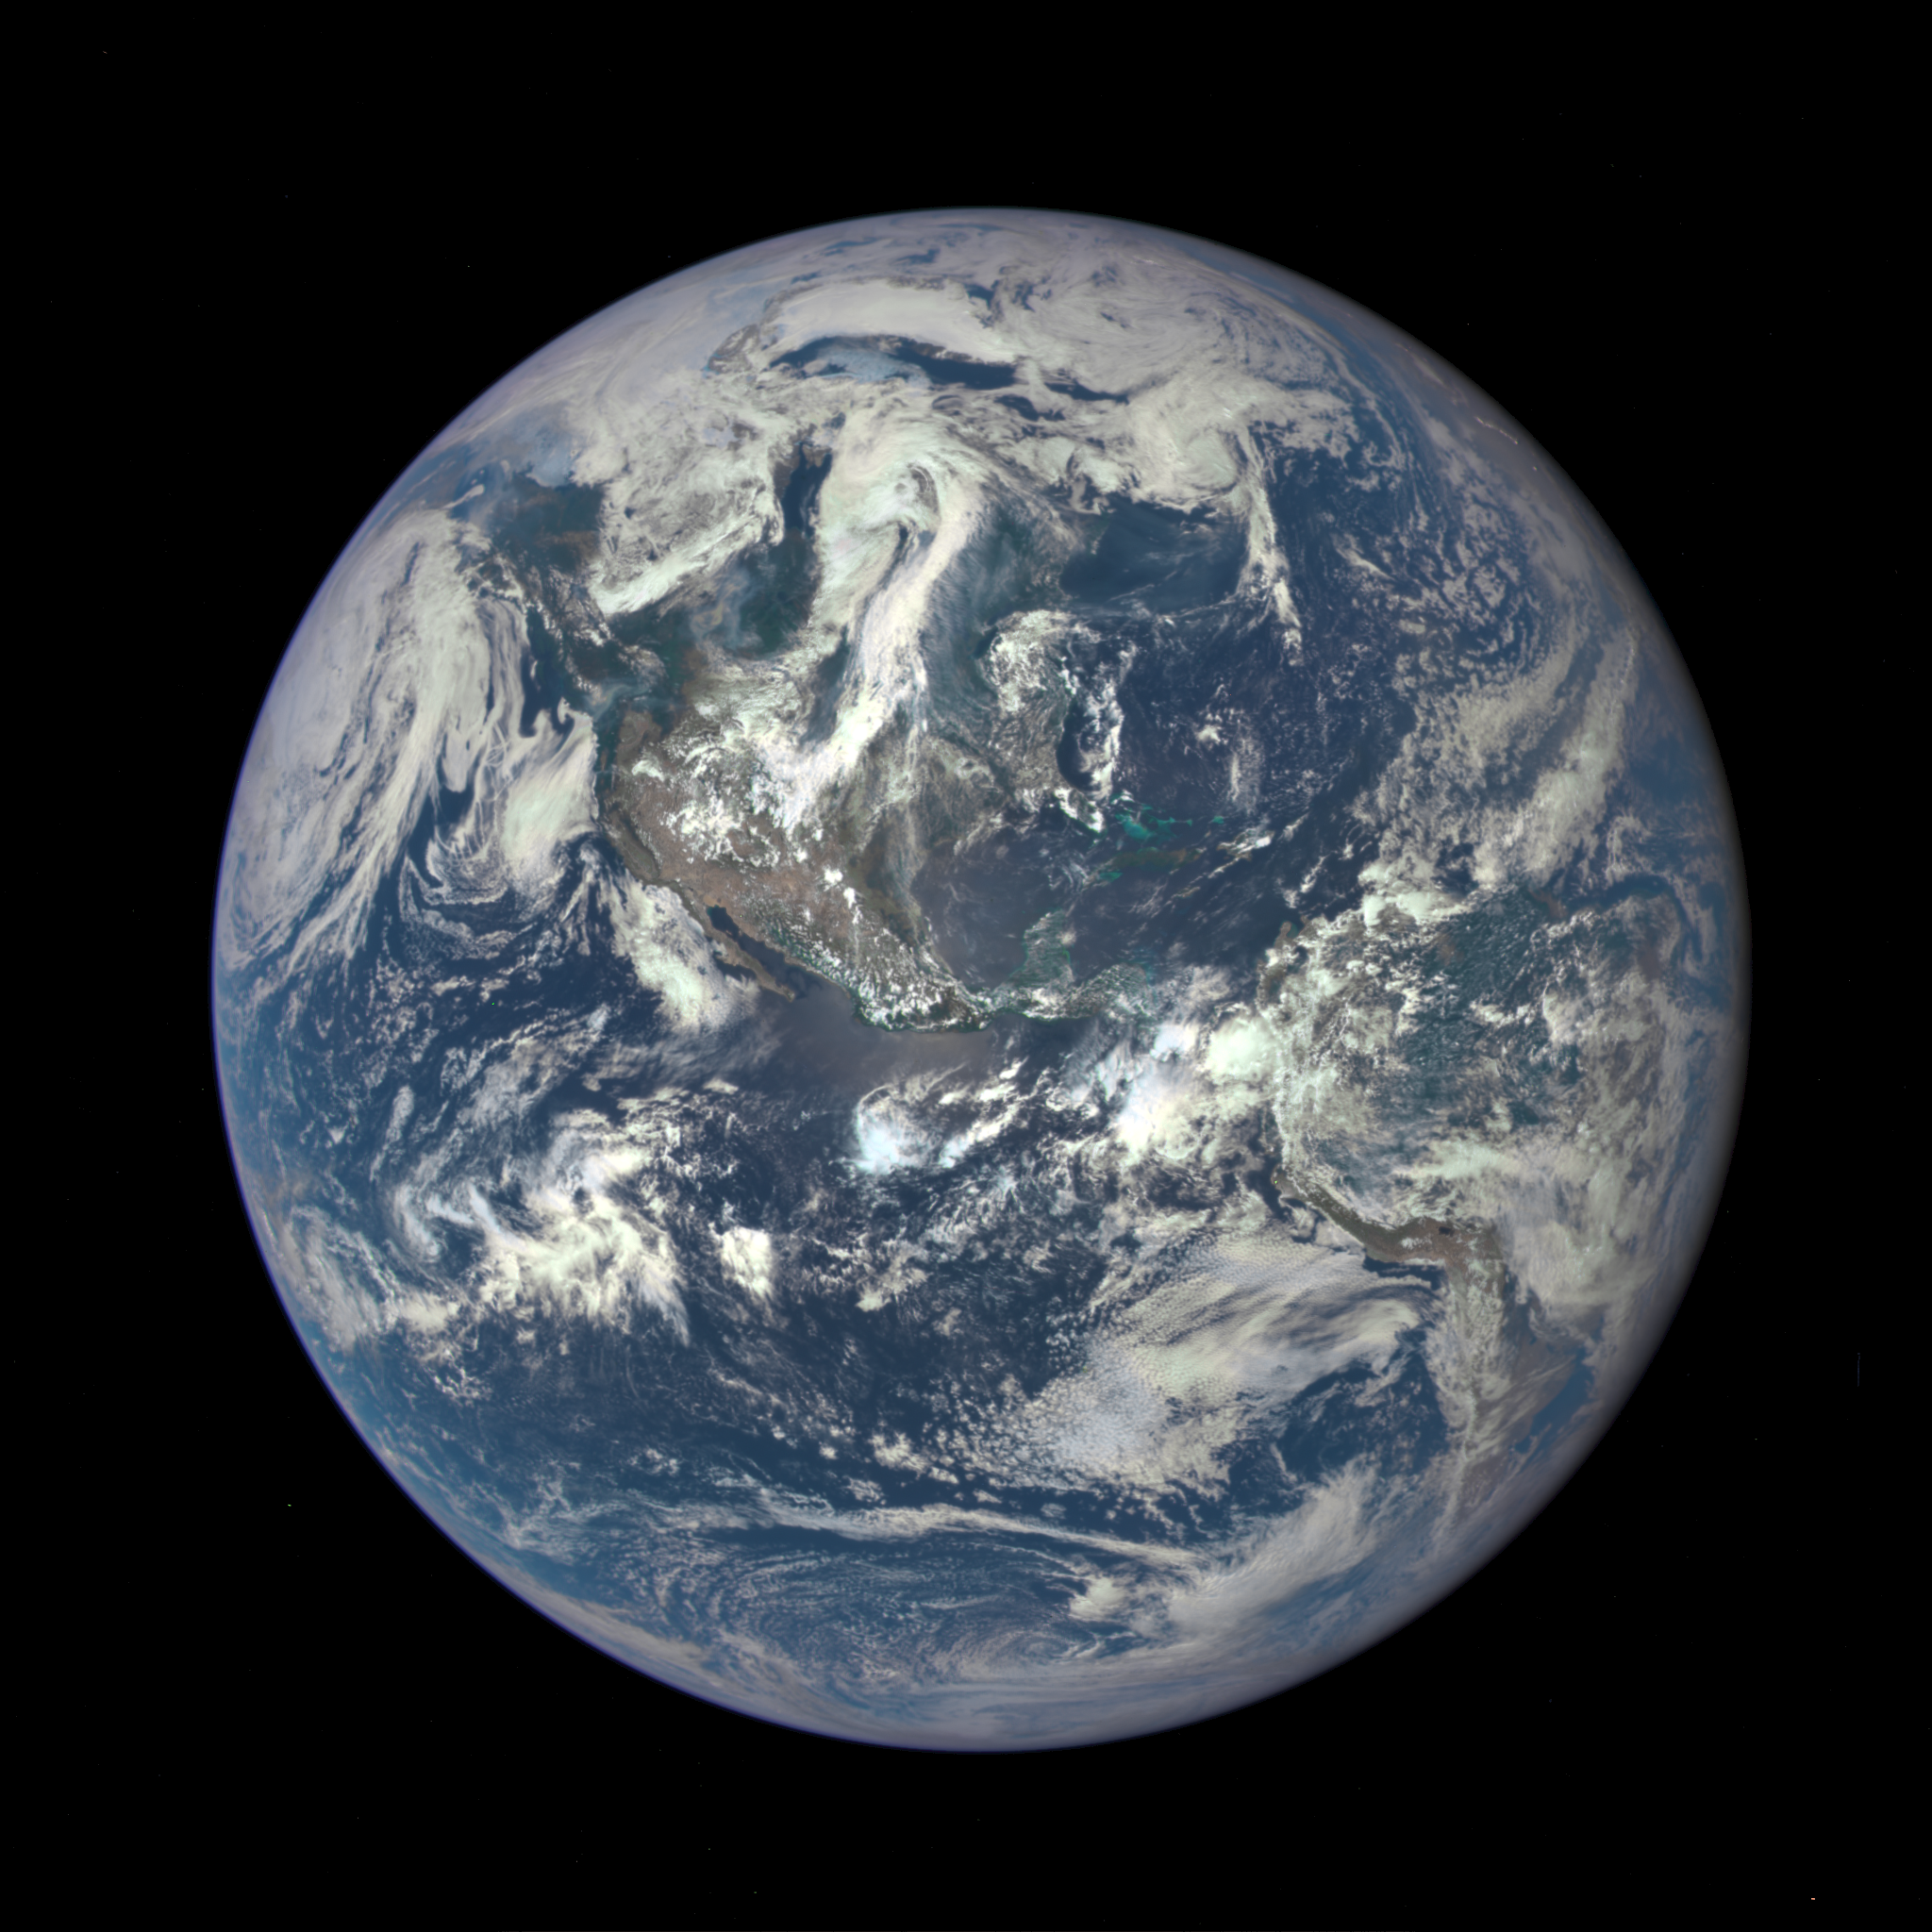
\includegraphics[width=3cm]{earth}
    \end{column}
    \begin{column}{6cm}
      {\footnotesize \begin{equation*}
          \begin{pmatrix}
            M_2 & -\frac{\Delta t}{2}D^T &
            -\frac{\Delta t}{2}Q\\[1ex]
            \frac{\Delta t}{2}c^2D & M_3 & 0\\[1ex]
            \frac{\Delta t}{2}N^2Q^T & 0 & M_b
          \end{pmatrix}
          \begin{pmatrix}
            \vec{U}\\[1ex]\vec{P}\\[1ex]\vec{B}
          \end{pmatrix}
          =
          \begin{pmatrix}
            M_2\vec{R}_u\\[1ex]
            M_3\vec{R}_p\\[1ex]
            M_b\vec{R}_b
          \end{pmatrix}
        \end{equation*}}
    \end{column}
  \end{columns}
  \begin{challenge}{Challenge}
    Invert elliptic operator fast enough for operational forecasting.

    High aspect ratio: black-box numerical solvers struggle.

    Need scalable, custom multigrid solver.
  \end{challenge}
\end{frame}
\begin{frame}
  \frametitle{Multigrid approach}
  \begin{columns}
    \begin{column}{0.5\textwidth}
      \begin{tikzpicture}
        \node (B) {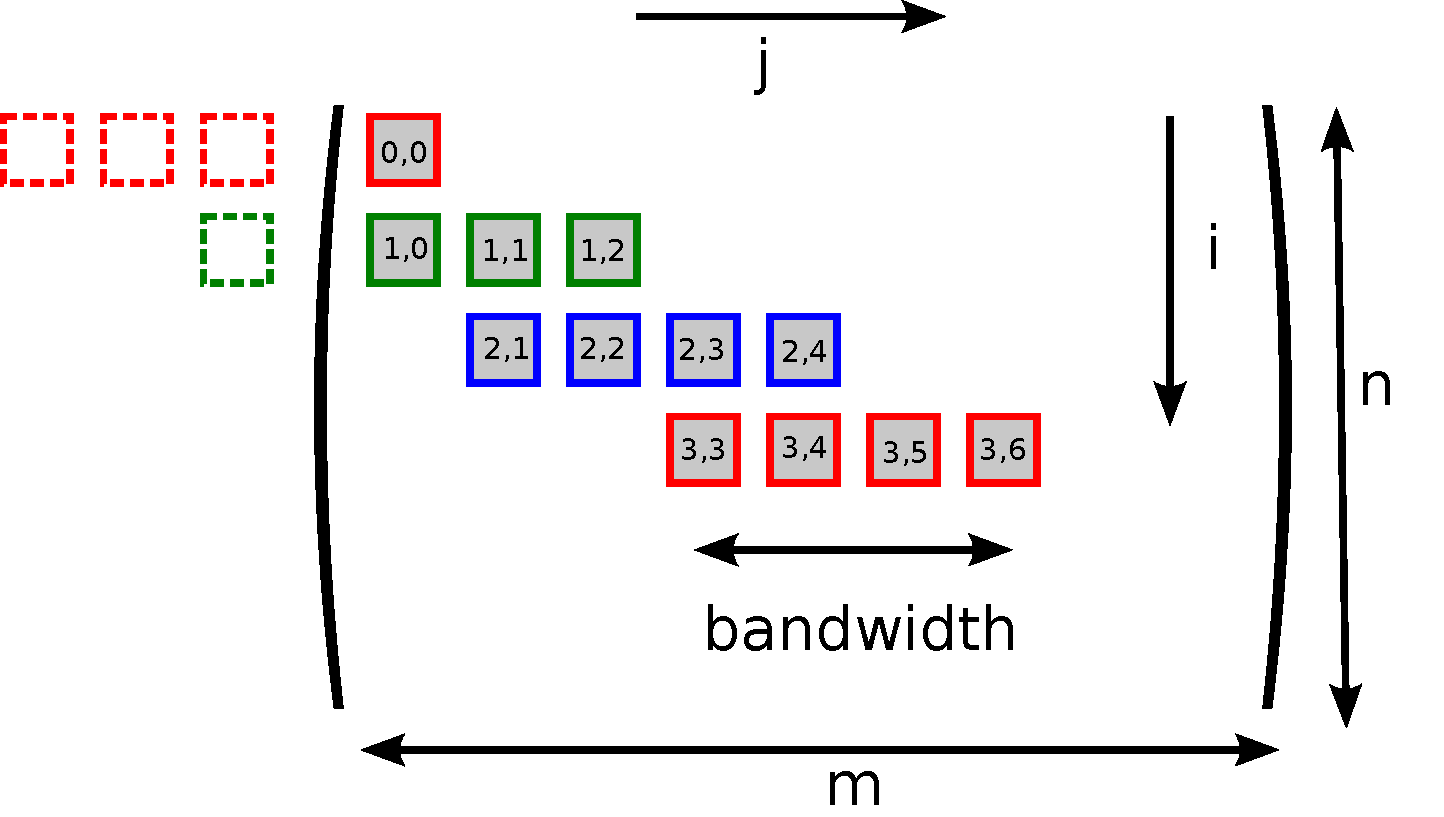
\includegraphics[height=1.5cm]{bandedmatrix}}; \node
        (C) [right=0.15cm of B,yshift=0.6cm]
        {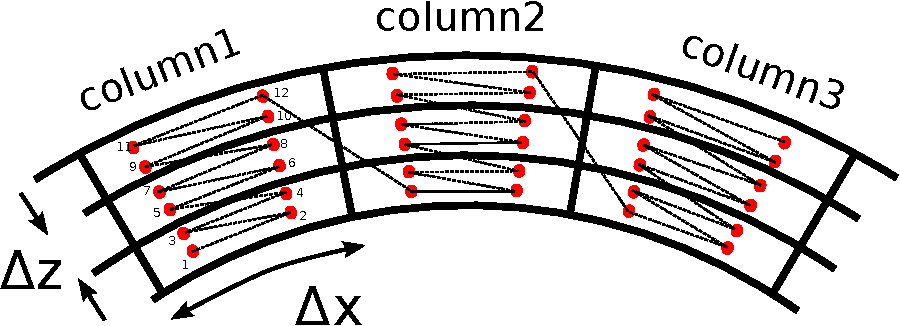
\includegraphics[height=1cm]{columndofs}}; \node (A)
        [below=0.05cm of C]
        {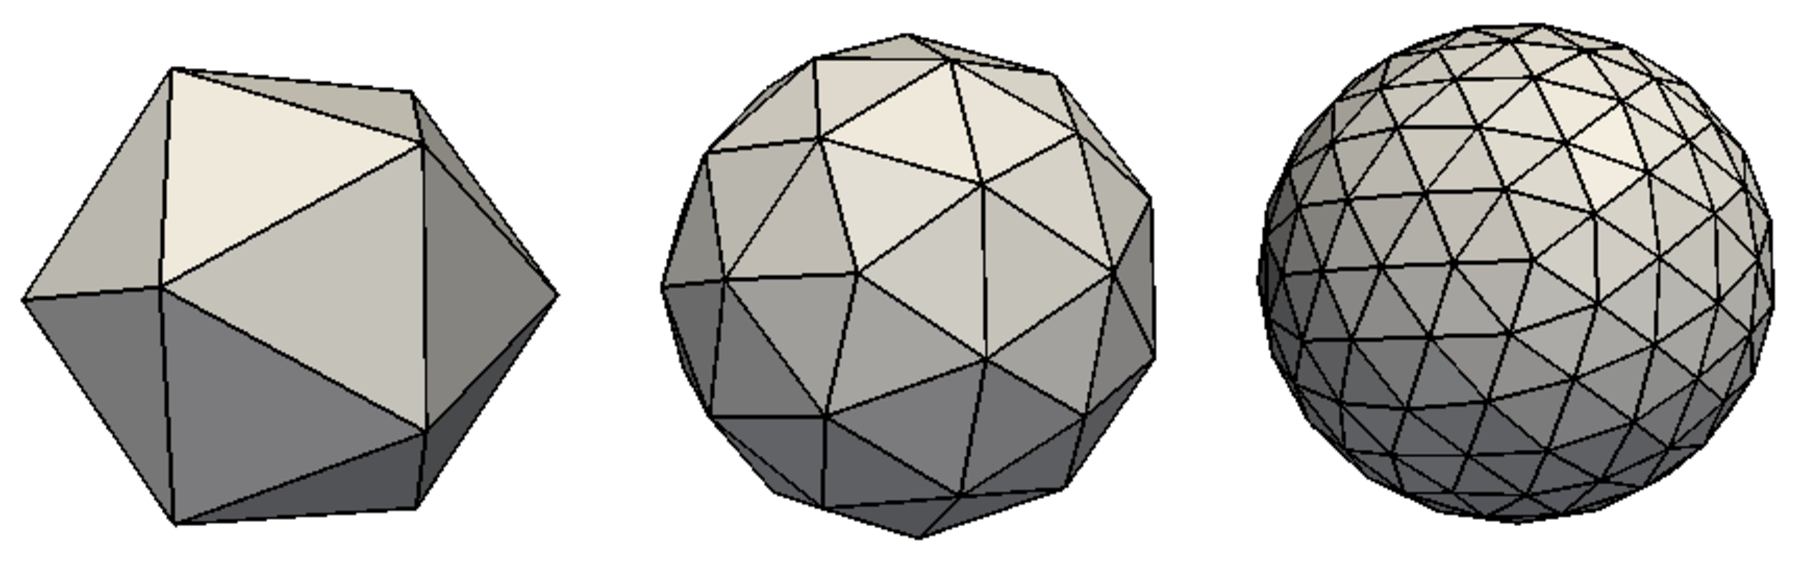
\includegraphics[height=0.75cm]{MeshHierarchy}};
      \end{tikzpicture}
    \end{column}
    \begin{column}{0.4\textwidth}
      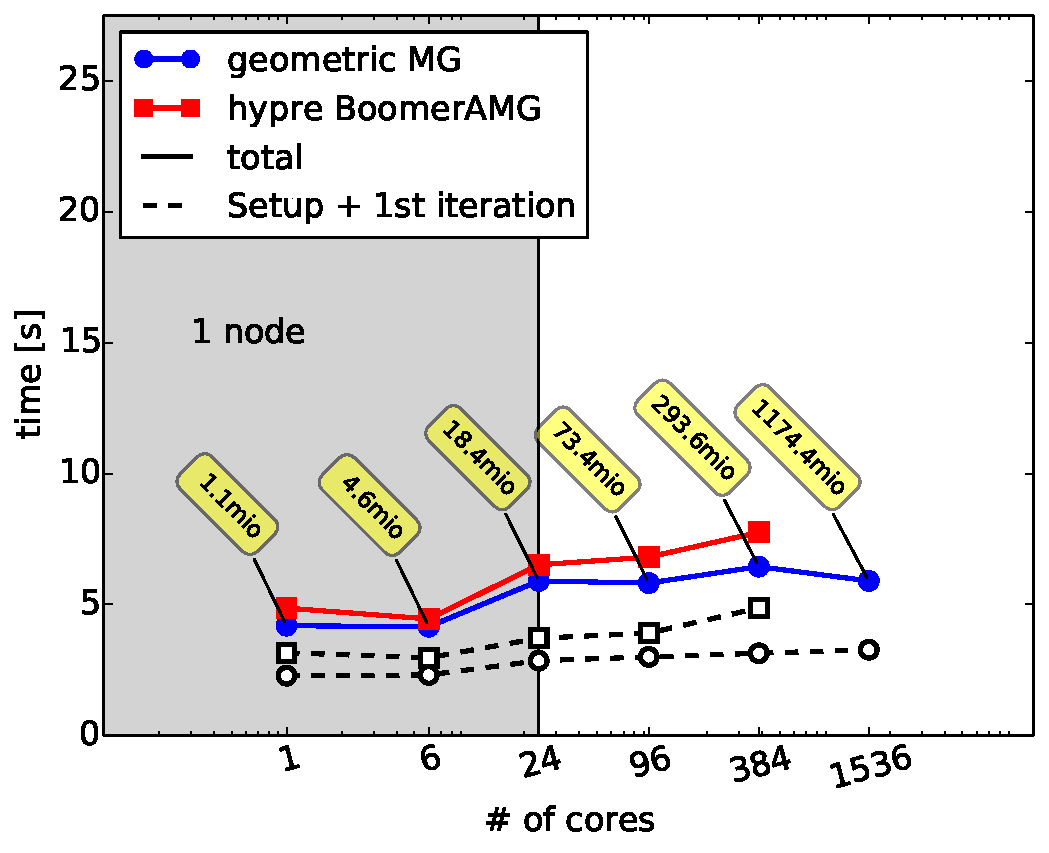
\includegraphics[width=4cm]{nwp-multigrid-scaling}
    \end{column}
  \end{columns}
    Developed custom tensor-product multigrid scheme, showed robustness
    and scalability.

    {\raggedleft\scriptsize\hfill \textbf{L.~Mitchell}, E.H.~M\"uller. JCP (2016). \arxivlink{1605.00492}{cs.MS}\nocite{Mitchell:2016}}
    \begin{block}{Future directions}
      Multilevel solvers for hybridised discretisations.

      Approach is being explored by UK Met Office in their next generation dynamical
      core.
    \end{block}
\end{frame}

\section{Preconditioning Navier--Stokes}

\begin{frame}
  \frametitle{Application challenge}
  \begin{block}{Stationary incompressible Navier--Stokes}
    For $\nu \in \mathbb{R}_+$, find $(u, p) \in \honev \times \ltwo$ such that
    \begin{alignat*}{2}
      - \div (2\nu\eps{u}) + \advect{u}{u} + \nabla p &= f \quad && \text{ in } \Omega, \label{eqn:momentum} \\
      \div u &= 0 \quad && \text{ in } \Omega, \\
      u &= g \quad && \text{ on } \Gamma_D, \\
      2 \nu \eps{u} \cdot n &= pn \quad && \text{ on } \Gamma_N,
    \end{alignat*}
  \end{block}
  \begin{answer}{Why?}
    Fully implicit discretisations of transient problem; bifurcation
    analysis of steady state.
  \end{answer}
\end{frame}

\begin{frame}
  \frametitle{Challenges for solvers}
  \begin{challenge}{Desired properties}
    \begin{itemize}
    \item Growth in time to solution is (at worst)
      $\mathcal{O}(n\log n)$ in number of degrees of freedom (resolution).
    \item Convergence does not degrade with $\nu \to 0$.
    \end{itemize}
  \end{challenge}
  \begin{columns}[t]
    \begin{column}{0.48\textwidth}
      \begin{block}{Direct methods}
        \begin{itemize}
        \item[\cmark] Convergence independent of $\nu$
        \item[\xmark] Time to solution $\mathcal{O}(n^2)$ (3D).
        \end{itemize}
      \end{block}
    \end{column}
    \begin{column}{0.48\textwidth}
      \begin{block}{Krylov methods}
        \begin{itemize}
        \item[\cmark] Time to solution $\mathcal{O}(n \log n)$ (with
          multilevel preconditioner)
        \item[\xmark] Convergence independent of $\nu$ challenging
        \end{itemize}
      \end{block}
    \end{column}
  \end{columns}
\end{frame}

\begin{frame}
  \frametitle{Block preconditioning}
  \begin{exampleblock}{Newton linearisation}
    \begin{equation*}
      P := \begin{pmatrix}
        A & B^T \\
        B & 0
      \end{pmatrix}
      \begin{pmatrix}
        \delta u \\ \delta p
      \end{pmatrix}
      =
      \begin{pmatrix}
        b \\ 0
      \end{pmatrix}.
    \end{equation*}
  \end{exampleblock}
  \pause
  \begin{answer}{Block factorisations}
    \begin{equation*}
      P^{-1} =
      \begin{pmatrix}
        I   & -A^{-1} B^T \\
        0 & I \\
      \end{pmatrix}
      \begin{pmatrix}
        A^{-1}  & 0 \\
        0 & S^{-1} \\
      \end{pmatrix}
      \begin{pmatrix}
        I   & 0 \\
        -BA^{-1} & I \\
      \end{pmatrix}
    \end{equation*}
  \end{answer}
  \begin{challenge}{PDE-specific challenge}
    Find good approximations $\tilde{A}^{-1}$ for $A^{-1}$ and
    $\tilde{S}^{-1}$ for $S^{-1}$.
  \end{challenge}
\end{frame}

\begin{frame}
  \frametitle{Choosing $\tilde{A}^{-1}$ and $\tilde{S}^{-1}$}
  \begin{exampleblock}{Stokes (no advection) \textcite{Silvester:1994}}
    Multigrid for $\tilde{A}^{-1}$, $\tilde{S}^{-1} = -\nu M_p^{-1}$
    \begin{itemize}
    \item[\cmark] $h$-independent
    \item[\xmark] Only effective up to $\Re \sim 10$ for Navier--Stokes.
    \end{itemize}
  \end{exampleblock}
  \begin{exampleblock}{PCD for Navier--Stokes \textcite{Kay:2002}}
    Multigrid for $\tilde{A}^{-1}$, approximate $\tilde{S}^{-1}$ with
    convection-diffusion solves on pressure space.
    \begin{itemize}
    \item[\cmark] $h$-independent
    \item[\xmark] Only effective up to $\Re \sim 100$-$1000$
    \end{itemize}
  \end{exampleblock}
\end{frame}

\begin{frame}
  \frametitle{Performance of pressure convection-diffusion (PCD)}
\begin{table}[htbp]
\centering
\begin{tabular}{cc|c@{\hspace{9pt}}c@{\hspace{9pt}}c}
\toprule
$1/h$ & \# degrees of freedom & \multicolumn{3}{c}{Reynolds number} \\
  && 10 & 100 & 1000 \\
\midrule
$2^4$ & $8.34 \times 10^2$ & 22.0 & 40.4 & 103.3 \\
$2^5$ & $3.20 \times 10^3$ & 23.0 & 41.3 & 137.7 \\
$2^6$ & $1.25 \times 10^4$ & 24.5 & 42.0 & 157.0 \\
$2^7$ & $4.97 \times 10^4$ & 25.5 & 42.7 & 149.0 \\
$2^8$ & $1.98 \times 10^5$ & 26.0 & 44.0 & 137.0 \\
\bottomrule
\end{tabular}
\caption{Average number of outer Krylov iterations per Newton step for the
2D regularized lid-driven cavity problem with PCD preconditioner.
Obtained with IFISS v3.5, $Q_1-P_0$ element pair.}
\label{tab:pcdlscldc}
\end{table}
\end{frame}

\begin{frame}
  \frametitle{Augmented Lagrangian approach}
  \begin{center}
    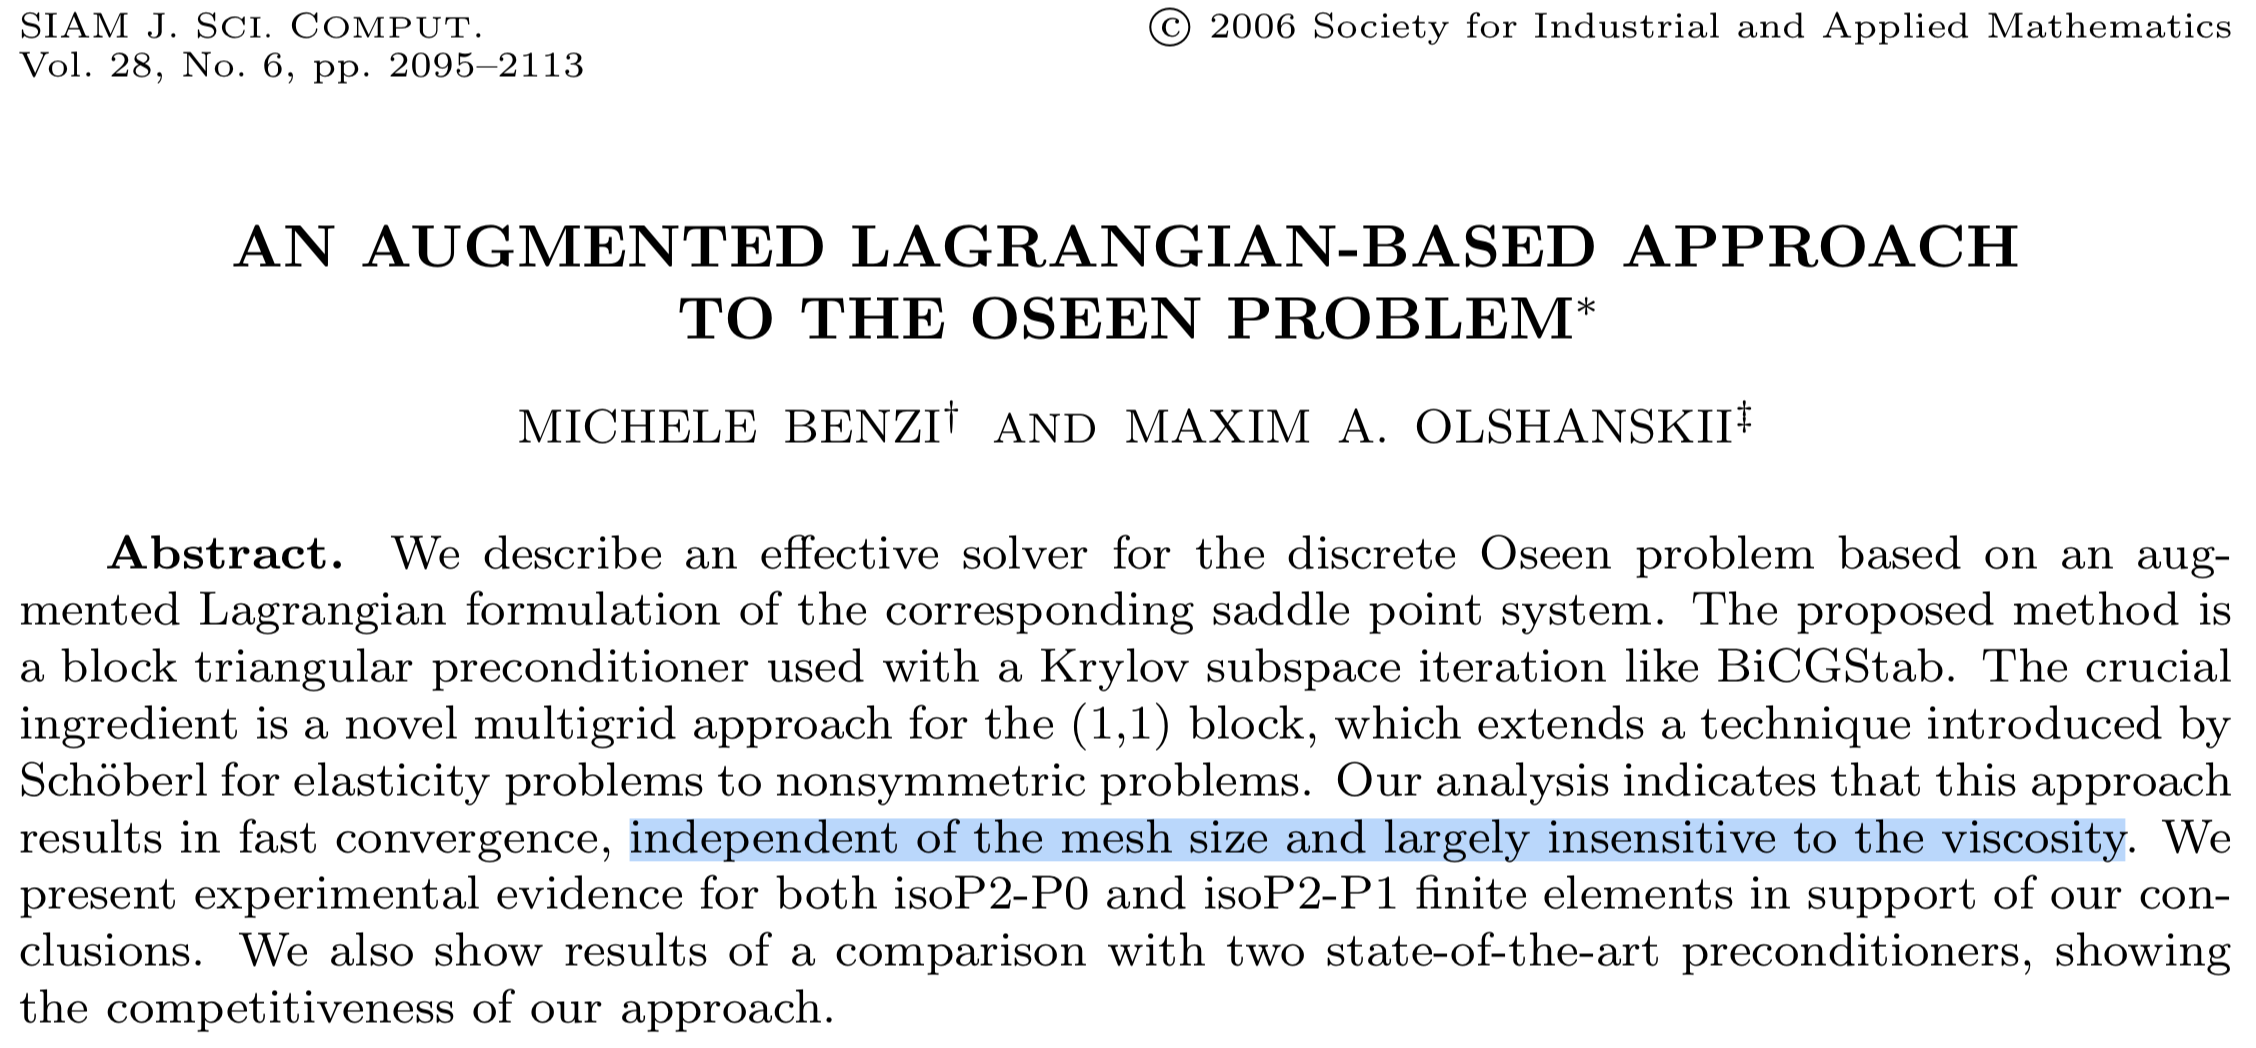
\includegraphics[width=\textwidth]{benzi06}
  \end{center}
  \pause
    \begin{block}{Observation}
    \begin{itemize}
    \item[\cmark] Viscosity-robust preconditioning
    \item[\xmark] Only 2D, no further implementation until 2018
    \end{itemize}
  \end{block}
\end{frame}
\begin{frame}[t]
  \frametitle{Objectives}
  \begin{itemize}
  \item First general implementation of the method. \cmark
  \item Extend the solver and discretisation to three dimensions. \cmark
  \item Extend approach to \emph{divergence-free} discretisations. \cmark
  \end{itemize}
  \begin{answer}{Three ideas}
    \begin{enumerate}
    \item Control Schur complement with an augmented Lagrangian term
    \item Kernel-capturing multigrid relaxation
    \item Robust multigrid prolongation
    \end{enumerate}
  \end{answer}
  {\hfill\raggedleft\scriptsize P.E.~Farrell, \textbf{L.~Mitchell}, F.~Wechsung. SIAM SISC (2019). \arxivlink{1810.03315}{math.NA}\nocite{Farrell:2019}}
\end{frame}

\begin{frame}
  \frametitle{Controlling the Schur complement}
  \begin{exampleblock}{Continuous augmentation}
    Add $\gamma \grad\div u$ term to the momentum equation.

    Doesn't change solution since $\div u = 0$
  \end{exampleblock}
  \begin{theorem}[Hestenes, Fortin, Glowinski, Olshanksii, \dots]
    As $\gamma \to \infty$, the Schur complement is well
    approximated by $\tilde{S}^{-1} = -(\nu + \gamma)M_p^{-1}$.
  \end{theorem}
  \pause
  \begin{exampleblock}{Discrete augmentation}
    \begin{equation*}
      \begin{pmatrix}
        A + \gamma B^T M_p^{-1} B & B^T \\
        B & 0
      \end{pmatrix}
      \begin{pmatrix}
        u \\ p
      \end{pmatrix}
      =
      \begin{pmatrix}
        b \\ 0
      \end{pmatrix}
    \end{equation*}

    Doesn't change solution since $B u = 0$.

    Again, as $\gamma \to \infty$, $S^{-1}$ is well approximated by
    $\tilde{S}^{-1} = -(\nu + \gamma)M_p^{-1}$.
  \end{exampleblock}
\end{frame}

\begin{frame}
  \frametitle{Conservation of misery}
  \begin{exampleblock}{Good news}
    The Schur complement becomes easy to approximate as $\gamma \to \infty$
  \end{exampleblock}
  \begin{challenge}{Bad news}
    Normal multigrid approaches for $\tilde{A}^{-1}$ don't work for
    $A_\gamma := A + \gamma B^T M_p^{-1} B$, and get \emph{worse} as
    $\gamma \to \infty$.
  \end{challenge}
  \pause
  \begin{center}
    \begin{tabular}{l| c |c}
      \toprule
      &  LU for $\tilde{A}_\gamma^{-1}$ & AMG for $\tilde{A}_\gamma^{-1}$\\
      \midrule
      $\gamma=10^{-1}$ & 15 &18\\
      $\gamma=1$ & 6 &40\\
      $\gamma=10^{1}$ & 3 &107\\
      \bottomrule
    \end{tabular}

    Outer Krylov iterations for different choices of $\tilde{A}^{-1}_\gamma$.
  \end{center}
\end{frame}


\begin{frame}
  \frametitle{Point smoother is not sufficient}
  \begin{itemize}
  \item Ignorning advection, then the top-left block corresponds to
    discretisation of
    \begin{equation*}
      a_{\gamma}(u, v) = \xunderbrace{\int_\Omega 2\nu \eps{u}  :
        \eps{v} \dx}_{\text{sym.~pos.~def.}} \quad +  \quad
      \textcolor{red}{\xunderbrace{\int_\Omega \gamma\div u\div v \dx}_{\text{sym.~pos.~semi-def.}}}
    \end{equation*}
    \pause
  \item The semi-definite term is singular on all solenoidal fields
    $\Rightarrow$ the system becomes \emph{nearly singular} as $\gamma
    \to \infty$
    \pause
  \item To build a $\gamma$-robust scheme we need
    \parencite{Schoeberl:1999}
    \begin{itemize}
    \item a $\gamma$-robust smoother;
    \item a prolongation operator with $\gamma$-independent continuity
      constant;
    \item[$\Rightarrow$] overlapping Schwarz smoother with
      decomposition that decomposes the kernel. ``The right blocks for
      block Jacobi''.
    \end{itemize}
  \end{itemize}
\end{frame}

\begin{frame}
  \frametitle{Discretisation requirements}
  \begin{itemize}
  \item Need inf-sup stable pair for velocity and pressure
  \item Need a \emph{local basis} for the kernel of div (for efficiency).
  \end{itemize}
  \begin{exampleblock}{Low-order}
    \begin{itemize}
    \item[2D] $P_2^2-P_0$
    \item[3D] $(P_1 \oplus \text{FB})^3-P_0$ ($\text{FB}$ cubic face bubbles)
    \item[$\Rightarrow$] overlapping \emph{star} patches
    \end{itemize}
  \begin{figure}
    \begin{center}
      
\includegraphics[width=6cm]{star}
    \end{center}
  \end{figure}
  \end{exampleblock}
\end{frame}

\begin{frame}
  \frametitle{Divergence-free pair}
  Choose element pair from discrete subcomplex of Stokes complex
  \begin{equation*}
    H^2 \xrightarrow{\grad} H^1(\curl) \xrightarrow{\curl} H^1 \xrightarrow{\div} L^2.
  \end{equation*}
  \vspace{-\baselineskip}
  \begin{exampleblock}{Divergence-free}
    \begin{itemize}
    \item Scott--Vogelius pair: $P_k^d-P_{k-1}^\text{disc}$ on barycentrically refined
      meshes ($k \ge d$).
    \end{itemize}
  \begin{figure}
    \begin{center}
      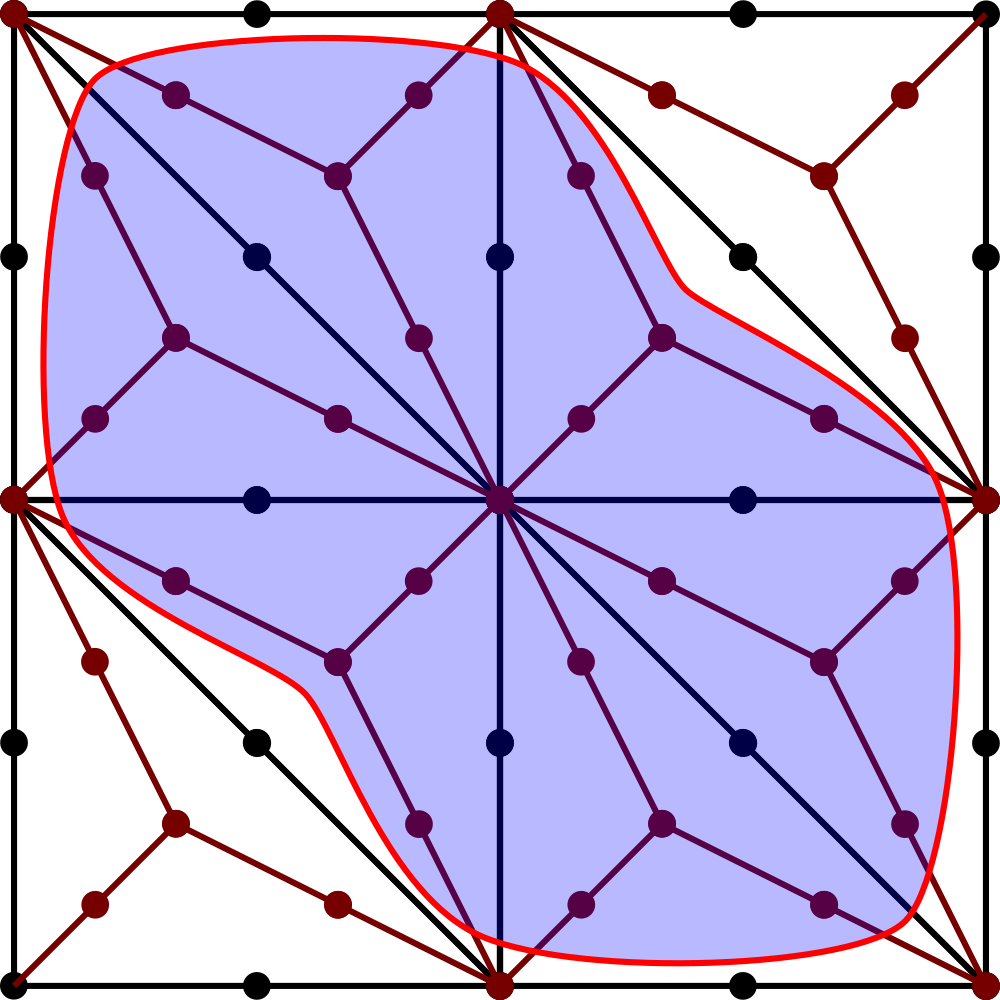
\includegraphics[width=6cm]{macrostar}
    \end{center}
  \end{figure}
  \end{exampleblock}
\end{frame}

\begin{frame}
  \frametitle{Numerical results --- 3D $(P_1 \oplus \text{FB})^3-P_0$}
  \begin{table}[htbp]
    \centering
    \begin{tabular}{cc|ccccc}
      \toprule
      \# ref. & \# dofs & \multicolumn{5}{c}{Reynolds number} \\
              && 10 & 100 & 1000 & 2500 & 5000 \\
      \midrule
      \multicolumn{7}{c}{Lid Driven Cavity}\\
      \midrule
      1 & $2.1 \times 10^6$ & 4.50 & 4.00 & 5.00 & 4.50 & 4.00 \\
      2 & $1.7 \times 10^7$ & 4.50 & 4.33 & 4.50 & 4.00 & 4.00 \\
      3 & $1.3 \times 10^8$ & 4.50 & 4.33 & 4.00 & 3.50 & 7.00 \\
      4 & $1.1 \times 10^9$ & 4.50 & 3.66 & 3.00 & 5.00 & 5.00 \\
      \midrule
      \multicolumn{7}{c}{Backwards facing step}\\
      \midrule
      1 & $2.1 \times 10^6$ & 4.50 & 4.00 & 4.00 & 4.50 & 7.50  \\
      2 & $1.7 \times 10^7$ & 5.00 & 4.00 & 3.33 & 4.00 & 10.00 \\
      3 & $1.3 \times 10^8$ & 6.50 & 4.50 & 3.50 & 3.00 & 8.00  \\
      4 & $1.0 \times 10^9$ & 7.50 & 3.50 & 2.50 & 3.00 & 6.00  \\
    \end{tabular}
    \caption{Average number of outer Krylov iterations per Newton step for two 3D benchmark problems.}
    \label{tab:ourldc3d}
  \end{table}
\end{frame}

\begin{frame}[t]
  \frametitle{Computational performance --- 3D}
  % [53.140734383333324, 68.56801668333334, 61.468243016666655, 65.64923281666665]
  \pgfplotstableread[col sep=comma, row sep=\\]{%
    Cores,Time,Dofs\\
    48,5.3e1,2134839\\
    384,6.9e1,16936779\\
    3072,6.1e1,134930451\\
    24576,6.6e1,1077196323\\
  }\ldctable
  % [55.02509561666667, 68.57286605, 57.029964033333336, 69.39903468333333]
  \pgfplotstableread[col sep=comma, row sep=\\]{%
    Cores,Time,Dofs\\
    48,5.5e1,2107839\\
    384,6.9e1,16534263\\
    3072,5.7e1,130973115\\
    24576,6.9e1,1042606515\\
  }\bfstable
  \begin{columns}
    \begin{column}{0.5\textwidth}
      \begin{center}
        \begin{tikzpicture}
          \begin{semilogxaxis}[
            width=0.955\linewidth,
            height=0.9\linewidth,
            log basis x=2,
            ymin=0,
            ymax=80,
            xtick=data,
            xticklabels from table={\ldctable}{Cores},
            extra x ticks={48, 384, 3072, 24576},
            extra x tick labels={$[2.13]$, $[16.9]$,$[135]$,$[1077]$},
            extra x tick style={tick label style={yshift=-2.5ex}},
            xlabel={Cores\\{}[DoFs $\times 10^6$]},
            xlabel style={align=center, style={yshift=-0.5ex}},
            ylabel near ticks,
            ylabel style={align=center, text width=4cm},
            title={3D lid-driven cavity.},
            ylabel={Time [min]},
            ]
            \addplot+ table[x=Cores,y=Time] {\ldctable};
          \end{semilogxaxis}
        \end{tikzpicture}
      \end{center}
    \end{column}
    \begin{column}{0.5\textwidth}
      {\centering
        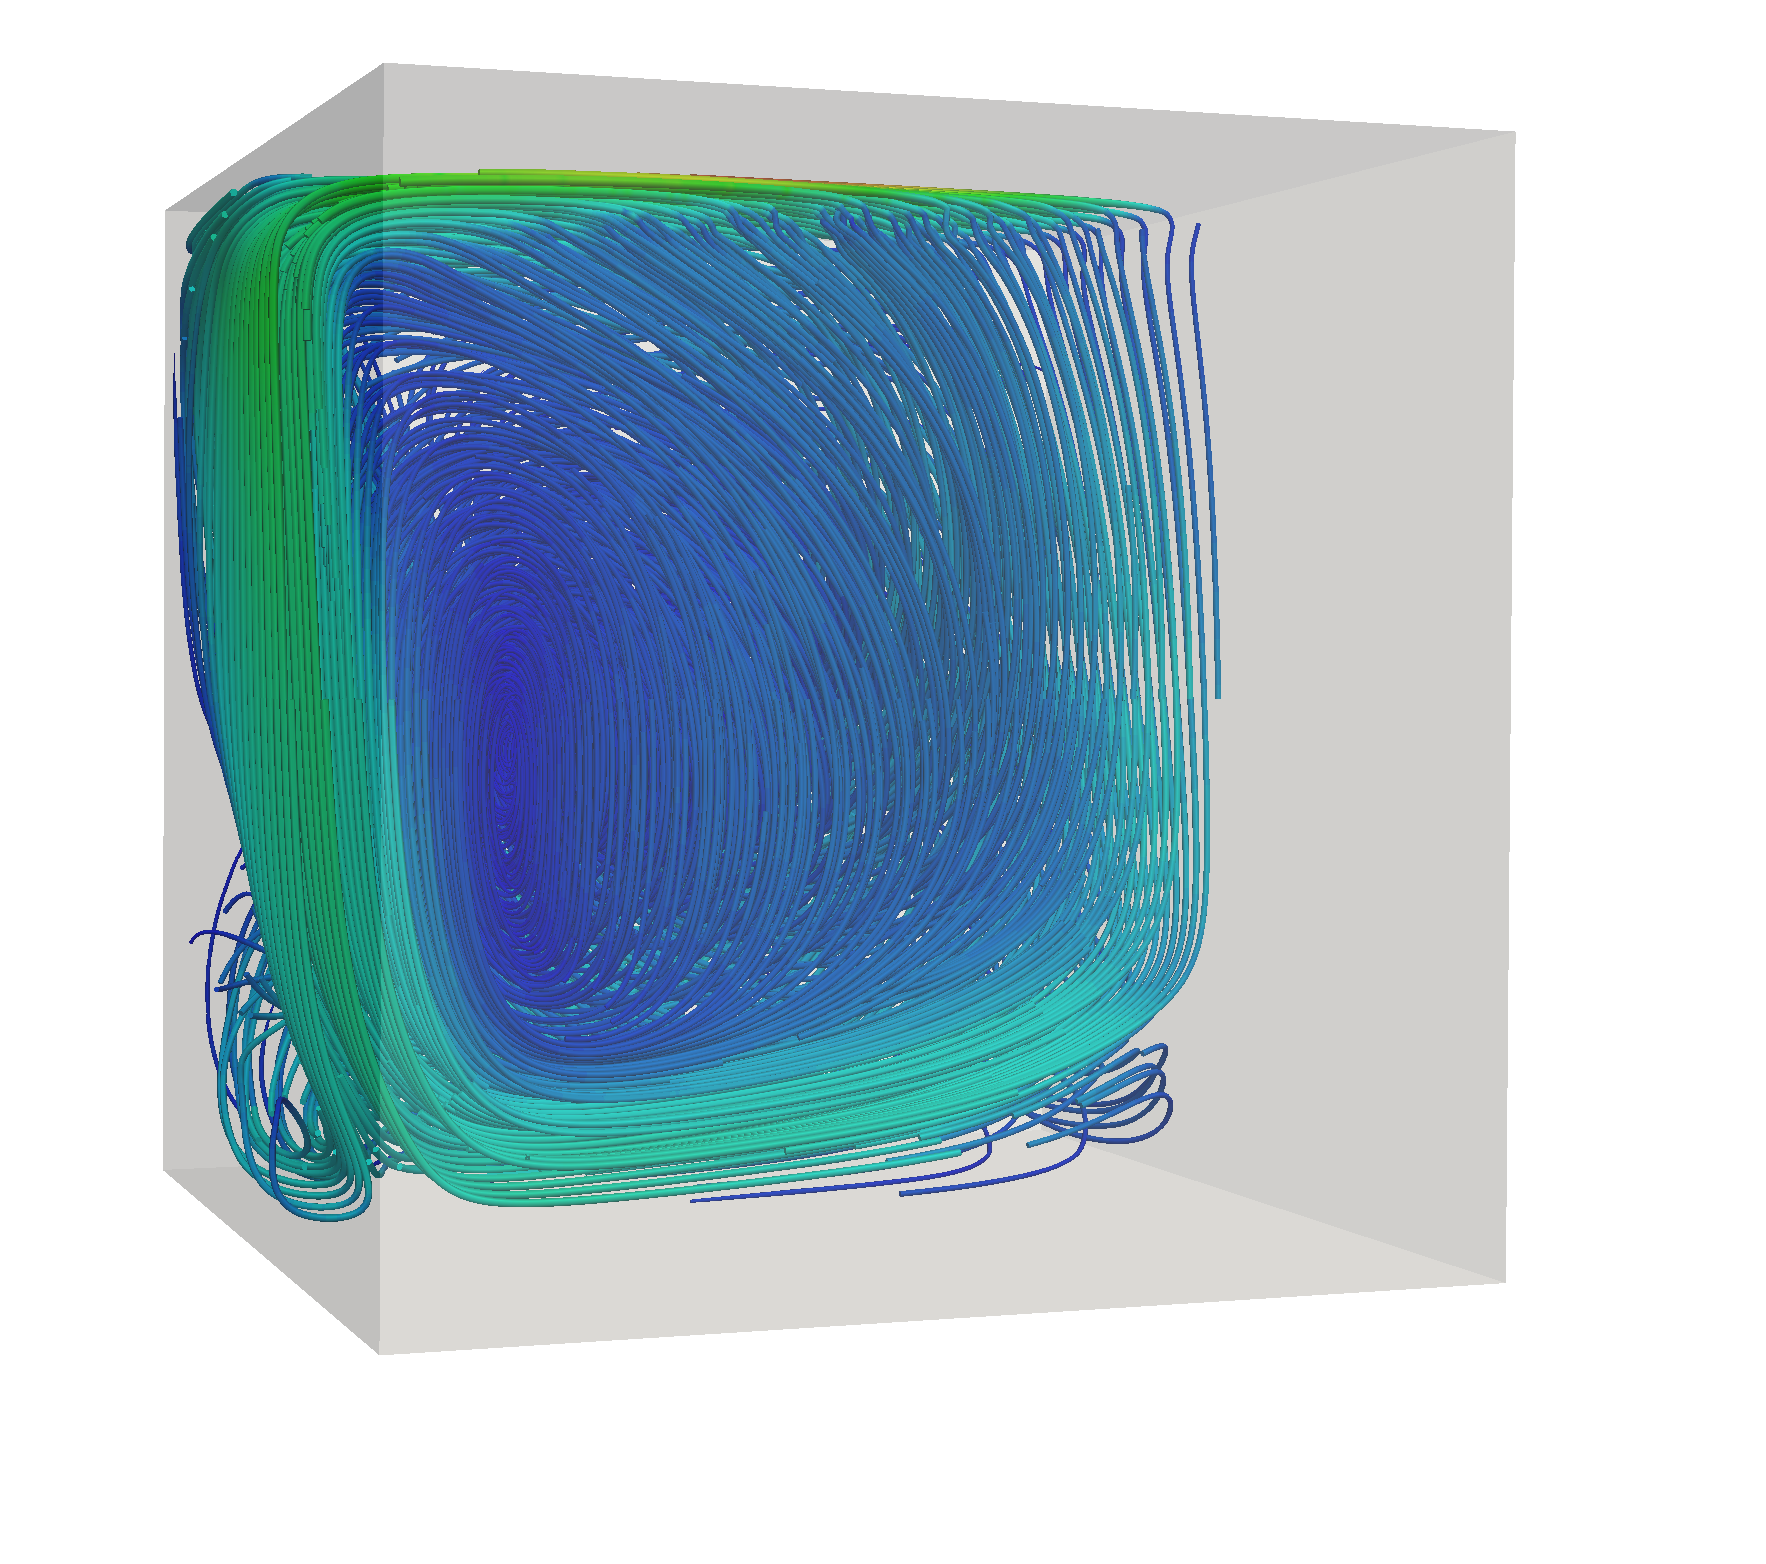
\includegraphics[width=\textwidth]{LDC-streamlines}}
      {\scriptsize Velocity streamlines at Reynolds number 5000.
        Credit F.~Wechsung, University of Oxford.}
    \end{column}
  \end{columns}
  \begin{center}
    50 continuation steps
  \end{center}
\end{frame}

\begin{frame}
  \frametitle{Numerical results --- 2D $P_3^2-P_2^\text{disc}$}
  \begin{table}[htbp]
    \centering
    \begin{tabular}{cc|ccccc}
      \toprule
      \# ref. & \# dofs & \multicolumn{5}{c}{Reynolds number} \\
              && 10 & 100 & 1000 & 5000 & 10000 \\
      \midrule
      \multicolumn{7}{c}{Lid Driven Cavity}\\
      \midrule
      1 & $9.3 \times 10^4$ & 2.50 & 2.33 & 2.33 & 5.50 & 8.50 \\
      2 & $3.7 \times 10^5$ & 2.00 & 2.00 & 2.00 & 4.00 & 6.00 \\
      3 & $1.5 \times 10^6$ & 2.00 & 1.67 & 1.67 & 2.50 & 3.50 \\
      4 & $5.9 \times 10^6$ & 2.00 & 1.67 & 1.50 & 1.50 & 4.00 \\
      \midrule
      \multicolumn{7}{c}{Backwards facing step}\\
      \midrule
      1 & $1.0 \times 10^6$ & 2.00 & 2.50 & 2.50 & 5.00 & 7.50  \\
      2 & $4.1 \times 10^6$ & 2.50 & 2.50 & 1.50 & 3.00 & 4.00 \\
      3 & $1.6 \times 10^7$ & 2.50 & 2.50 & 1.50 & 1.50 & 2.50  \\
    \end{tabular}
    \caption{Average number of outer Krylov iterations per Newton step for two 2D benchmark problems.}
  \end{table}
\end{frame}

\begin{frame}
  \frametitle{Main result}
  \begin{exampleblock}{}
    It is possible to solve the Navier--Stokes equations in a Reynolds-robust way!

    Even for exactly divergence-free discretisations.

    {\hfill\scriptsize\raggedleft Open source implementation at \url{https://github.com/florianwechsung/alfi}}
  \end{exampleblock}
  \begin{answer}{Enabling mathematical software}
    General implementation enabled by new mathematical software
    developments:
    \begin{itemize}
    \item Extensible block-preconditioning framework in Firedrake

      {\hfill\scriptsize\raggedleft R.C.~Kirby, \textbf{L.~Mitchell}. SIAM
        SISC (2018). \arxivlink{1706.01346}{cs.MS}\nocite{Kirby:2018}}
    \item New preconditioner in PETSc and Firedrake for multigrid relaxation schemes based on
      subspace correction methods

      {\hfill\scriptsize\raggedleft P.E.~Farrell, M.G.~Knepley,
        \textbf{L.~Mitchell}, F.~Wechsung. \arxivlink{1912.08516}{cs.MS}\nocite{Farrell:2019b}}
    \end{itemize}
  \end{answer}
\end{frame}

\section{Future directions}

\begin{frame}
  \begin{block}{Idea}
    \begin{itemize}
    \item Mathematics is the language used to derive optimal solvers.

    \item It \emph{should be} the language we use to describe their implementation.
    \end{itemize}
  \end{block}
  \begin{challenge}{Challenges}
    \begin{itemize}
    \item Is there appropriate language to describe these problems to a
      computer?
    \item Not everything is a PDE, what then?
    \end{itemize}
  \end{challenge}
  \begin{answer}{Rewards}
    \begin{itemize}
    \item Bring state-of-the-art numerical solvers to the masses.
    \item Enable more exploratory, and creative, mathematics.
    \end{itemize}
  \end{answer}
\end{frame}

\begin{frame}
  \frametitle{Summary}
  \begin{itemize}
  \item Broad interdisciplinary research agenda spanning:
    \begin{itemize}
    \item finite element discretisation and implementation;
    \item linear and non-linear solvers/preconditioners;
    \item high-performance computing;
    \item domain-specific compilers.
    \end{itemize}
  \item Application areas:
    \begin{itemize}
    \item coastal ocean \& freshwater outflow;
    \item renewable energy;
    \item numerical weather prediction.
    \end{itemize}
  \end{itemize}
\end{frame}

\appendix
\begin{frame}[t,allowframebreaks]
  \frametitle{References}
  \printbibliography[heading=none]
\end{frame}

\end{document}
